\documentclass[a4paper,12pt]{article}
%%%%%%%%%%%%%%%%%%%%%%%%%%%%%%%%%%%%%%%%%%%%%%%%%%%%%%%%%%%%%%%%%%%%%%%%%%%%%%%%%%%%%%%%%%%%%%%%%%%%%%%%%%%%%%%%%%%%%%%%%%%%%%%%%%%%%%%%%%%%%%%%%%%%%%%%%%%%%%%%%%%%%%%%%%%%%%%%%%%%%%%%%%%%%%%%%%%%%%%%%%%%%%%%%%%%%%%%%%%%%%%%%%%%%%%%%%%%%%%%%%%%%%%%%%%%
\usepackage{eurosym}
\usepackage{vmargin}
\usepackage{amsmath}
\usepackage{graphics}
\usepackage{epsfig}
\usepackage{subfigure}
\usepackage{fancyhdr}
%\usepackage{listings}
\usepackage{framed}
\usepackage{graphicx}

\setcounter{MaxMatrixCols}{10}
%TCIDATA{OutputFilter=LATEX.DLL}
%TCIDATA{Version=5.00.0.2570}
%TCIDATA{<META NAME="SaveForMode" CONTENT="1">}
%TCIDATA{LastRevised=Wednesday, February 23, 2011 13:24:34}
%TCIDATA{<META NAME="GraphicsSave" CONTENT="32">}
%TCIDATA{Language=American English}

\pagestyle{fancy}
\setmarginsrb{20mm}{0mm}{20mm}{25mm}{12mm}{11mm}{0mm}{11mm}
\lhead{MA4128} \rhead{Mr. Kevin O'Brien}
\chead{Advanced Data Modelling}
%\input{tcilatex}


% http://www.norusis.com/pdf/SPC_v13.pdf
\begin{document}


%SESSION 1: Hierarchical Clustering
% Hierarchical clustering - dendrograms
% Divisive vs. agglomerative methods
% Different linkage methods

%SESSION 2: K-means Clustering

\tableofcontents
\newpage

\section{Introduction to Cluster Analysis}


%Introduction
Cluster analysis is a major technique for classifying a large volumes of information into
manageable meaningful piles. Cluster analysis is a data reduction tool that creates subgroups that are
more manageable than individual data items. In other words cluster analysis is an exploratory data analysis tool which aims at sorting different objects into groups in a way that the degree of association between two objects is maximal if they belong to the same group and minimal otherwise. Given the above, cluster analysis can be used to discover structures in data without providing an explanation/interpretation. In other words, cluster analysis simply discovers structures in data without explaining why they exist. Like factor analysis, it examines the full complement
of inter-relationships between variables. Both cluster analysis (and later, discriminant
analysis) are concerned with classification.

However, the latter requires prior knowledge of membership of each cluster in order to classify new cases. In cluster analysis
there is no prior knowledge about which elements belong to which clusters. The grouping
or clusters are defined through an analysis of the data. Subsequent multivariate analyses
can be performed on the clusters as groups.

\textbf{\textit{A cluster is a group of relatively homogeneous cases or observations.}}


The term cluster analysis encompasses a number of different algorithms and methods for grouping objects of similar kind into respective categories.A general question facing researchers in many areas of inquiry is how to organize observed data into meaningful structures, that is, to develop \textbf{\emph{taxonomies}}.

\subsection{Applications of Cluster Analysis}

We deal with clustering in almost every aspect of daily life. For example, a group of diners sharing the same table in a restaurant may be regarded as a cluster of people. In food stores items of similar nature, such as different types of meat or vegetables are displayed in the same or nearby locations. There is a countless number of examples in which clustering plays an important role. Clustering techniques have been applied to a wide variety of scientific research problems. For example, in the field of medicine, clustering diseases, cures for diseases, or symptoms of diseases can lead to very useful taxonomies. In the field of psychiatry, the correct diagnosis of clusters of symptoms such as paranoia, schizophrenia, etc. is essential for successful therapy. In archeology, researchers have attempted to establish taxonomies of stone tools, funeral objects, etc. by applying cluster analytic techniques. According to the modern system employed in biology, man belongs to the primates, the mammals, the amniotes, the vertebrates, and the animals.

Note how in this classification, the higher the level of aggregation the less similar are the members in the respective class. Man has more in common with all other primates (e.g., apes) than it does with the more "distant" members of the mammals (e.g., dogs), etc.

In general, whenever we need to classify a "mountain" of information into manageable meaningful piles, cluster analysis is of great utility.


%---------------------------------------------------------------%
\section{Cluster Analysis Techniques}
Cluster analysis (CA) is an exploratory data analysis tool for organizing observed data into meaningful taxonomies, groups, or
clusters, based on combinations of independent variables, which maximizes the similarity of cases within
each cluster while maximizing the dissimilarity between groups that are initially unknown.

In this sense, CA creates new groupings without any preconceived notion of what clusters
may arise, whereas \textit{\textbf{discriminant analysis}} classifies people and items into
already known groups.

CA provides no explanation as to why the clusters exist nor is any
interpretation made. Each cluster thus describes, in terms of the data collected, the class to
which its members belong. Items in each cluster are similar in some ways to each other and
dissimilar to those in other clusters.

Cluster analysis is a tool of discovery revealing associations and structure in data which, though not previously
evident, are sensible and useful when discovered. Importantly, CA enables new
cases to be assigned to classes for identification and diagnostic purposes; or find \textbf{\textit{exemplars}}
to represent classes.

\subsection{Types of Cluster Analysis}
There are three main types of cluster analysis.
\begin{itemize}
\item Hierarchical Clustering Analysis
\item Non-hierarchical Clustering Analysis (K-means clustering)
\item Two Step Clustering Analysis
\end{itemize}

Within hierarchical clustering analysis there are two subcategories: 
\begin{itemize}
\item Agglomerative (start from n clusters,to get to 1 cluster)
\item Divisive (start from 1 cluster, to get to $n$ cluster)
\end{itemize}


%---------------------------------------------------------------------------------%
\subsection{Hierarchical cluster analysis}
This is the major statistical method for finding relatively homogeneous clusters of cases based on measured characteristics.

Agglomerative clustering starts with each case as a separate cluster, i.e. there are as many clusters as cases, and then combines the clusters sequentially, reducing the number of clusters at each step until only one cluster is left.

The clustering method uses the dissimilarities or distances between objects when forming the clusters. The SPSS programme calculates \textbf{\textit{distances}} between data points in terms of the specified variables.

A hierarchical tree diagram, called a \textbf{\textit{dendrogram }} on SPSS, can be produced to show the linkage points. The clusters are linked at increasing levels of \textbf{\textit{dissimilarity}}.
The actual measure of dissimilarity depends on the measure used.


\subsection{Distance measures}
Distance can be measured in a variety of ways. There are distances that are Euclidean (can be measured with a ruler) and there are other distances based on similarity. For example, in terms of
geographical distance (i.e. Euclidean distance) Perth, Australia is closer to Jakarta, Indonesia, than it is to Sydney, Australia.

However, if distance is measured in terms of the cities characteristics, Perth is closer to Sydney (e.g. both on a big river estuary, straddling both sides of the river, with surfing beaches, and both English speaking, etc). A number of distance measures are available within SPSS. The \textbf{\textit{squared Euclidean distance}} is the most widely used measure.

\subsection{Squared Euclidean distance}
The most straightforward and generally accepted way of computing distances between objects in a multi-dimensional space is to compute Euclidean distances, an extension of Pythagoras's theorem.
If we had a two- or three-dimensional space this measure is the actual geometric distance between objects in the space (i.e. as if measured with a ruler).

In a univariate example, the Euclidean distance between two values is the arithmetic difference, i.e. \textbf{\textit{value1 - value2}}. In the bivariate case, the minimum distance is the hypotenuse of a triangle formed from the points, as in Pythagoras's theorem.

Although difficult to visualize, an extension of the Pythagoras's theorem will give the distance between two points in n-dimensional space. The squared Euclidean distance is used more often than the simple Euclidean distance in order to place progressively greater weight on objects that are further apart. Euclidean (and squared Euclidean) distances are usually computed from raw data, and not from transformed data, e.g. standardized data.

\subsection{Statistical Significance Testing}

Note that the previous discussions refer to clustering algorithms and do not mention anything about statistical significance testing. In fact, cluster analysis is not as much a typical statistical test as it is a ``collection" of different algorithms that ``put objects into clusters according to well defined similarity rules."

The point here is that, unlike many other statistical procedures, cluster analysis methods are mostly used when we do not have any \textbf{\textit{a priori hypotheses}}, but are still in the exploratory phase of our research. In a sense, cluster analysis finds the ``most significant solution possible." Therefore, statistical significance testing is really not appropriate here, even in cases when p-values are reported.

\subsection{Dendrograms}

The dendrogram is a tree-structured graphical representation, used to visualize of the results of \textbf{\textit{hierarchical cluster analysis}} . This is a tree-like plot where each step of hierarchical clustering is represented as a joining (or fusion) of two branches of the tree into a single one. The branches represent clusters obtained on each step of hierarchical clustering. The result of a clustering is presented either as the \textbf{\textit{distance}} or the similarity between the clustered rows or columns depending on the selected distance measure.


%----------------------------------------------------------%
% http://www2.statistics.com/resources/glossary/h/hclusteran.php

% http://mlsc.lboro.ac.uk/resources/statistics/Clusteranalysis.pdf

\section{Cluster Methods}
Having selected how we will measure distance, we must now choose the clustering algorithm, i.e. the rules that govern between which points distances are measured to determine cluster membership. There are many methods available, the criteria used differ and hence
different classifications may be obtained for the same data. This is important since it tells us that, although cluster analysis may provide an objective method for the clustering of cases, there can be subjectivity in the choice of method. 

The linkage distances are calculated by SPSS. The goal of the clustering algorithm is to join objects together into successively larger clusters, using some measure of similarity or distance. SPSS provides seven clustering algorithms, the most commonly used one being  \textbf{\textit{Ward's method}}.


\subsection{Nearest neighbour method} 
(Also known as the single linkage method).\\
In this method the distance between two clusters is defined to be the distance between
the two closest members, or neighbours. This method is relatively simple but is often
criticised because it doesn�t take account of cluster structure and can result in a problem
called chaining whereby clusters end up being long and straggly. However, it is better
than the other methods when the natural clusters are not spherical or elliptical in shape.

\subsection{Furthest neighbour method}
(Also known as the complete linkage method).\\
In this case the distance between two clusters is defined to be the maximum distance
between members  i.e. the distance between the two subjects that are furthest apart.
This method tends to produce compact clusters of similar size but, as for the nearest
neighbour method, does not take account of cluster structure. It is also quite sensitive
to outliers.

\subsection{Average (between groups) linkage method }
(sometimes referred to as UPGMA).\\
The distance between two clusters is calculated as the average distance between all pairs
of subjects in the two clusters. This is considered to be a fairly robust method.

\subsection{Centroid method}
Here the centroid (mean value for each variable) of each cluster is calculated and the
distance between centroids is used. Clusters whose centroids are closest together are
merged. This method is also fairly robust.

\subsection{Ward�s method}
In this method all possible pairs of clusters are combined and the sum of the squared
distances within each cluster is calculated. This is then summed over all clusters. The
combination that gives the lowest sum of squares is chosen. This method tends to
produce clusters of approximately equal size, which is not always desirable. It is also
quite sensitive to outliers. Despite this, it is one of the most popular methods, along
with the average linkage method.

%\subsection{Ward's Method}
%This method is distinct from other methods because it uses an \textbf{\textit{analysis of variance}} approach to evaluate the distances between clusters. In general, this method is very efficient.
%
%Cluster membership is assessed by calculating the total sum of squared deviations from the mean of a cluster. The criterion for fusion is that it should produce the smallest possible increase
%in the error sum of squares.
%
%
%
%\subsection{Ward's Linkage}
%
%Ward's linkage is a method for hierarchical cluster analysis . The idea has much in common with analysis of variance (ANOVA). The linkage function specifying the distance between two clusters is computed as the increase in the "error sum of squares" (ESS) after fusing two clusters into a single cluster. Ward's Method seeks to choose the successive clustering steps so as to minimize the increase in ESS at each step.


%
%\subsection{Applications of Cluster Analysis}
%
%In medicine, the clustering of symptoms and diseases leads to taxonomies of illnesses. In the field of business, clusters of consumer segments are often sought for successful marketing strategies. Biologists have to organize the different species of animals before a meaningful description of the differences between animals is possible.

%\subsection{Cluster Analysis as a Statistical Tool}



\section{Simple Case Studies}
\subsection{Market Segmentation}
Suppose a market research company wants to undertake direct mail advertising with specific advertisements
for different groups of people. You could use a variety of independent variabless like \textbf{\textit{family income}}
, \textbf{\textit{age}}, \textbf{\textit{number of cars per family}}, \textbf{\textit{number of mobile phones per family}},\textbf{\textit{number of school children per family}}  etc., to see if different postal or zip codes are characterized by particular combinations of demographic variables which could be grouped together to create a better way of directing the mail out.

This firm might in fact find that postal codes could be grouped into a number of clusters, characterized as ``the retirement zone", ``nappy valley", ``the golf club set", the ``rottweiler in a pick-up" district, etc. This sort of grouping might  be valuable in deciding where to place several new wine stores, or `Tummy to Toddler" shops.

Using cluster analysis, a customer ``type" can represent a homogeneous market segment.
Identifying their particular needs in that market allows products to be designed with greater
precision and direct appeal within the segment. Targeting specific segments is cheaper and
more accurate than broad-scale marketing. Customers respond better to segment marketing
which addresses their specific needs, leading to increased market share and customer
retention.

This is valuable, for example, in banking, insurance and tourism markets. Suppose
four clusters or market segments in the vacation travel industry. They are:
\begin{itemize}
\item[(1)] The high spending elite - they want top level service and expect to be pampered;
\item[(2)] The escapists - they want to get away and just relax;
\item[(3)] The educationalist - they want to see new things, go to museums,
have a safari, or experience new cultures;
\item[(4)] the sports person - they want the golf course, tennis court, surfing, deep-sea fishing, climbing, etc.
\end{itemize}
Different brochures and advertising is required for each of these.

Brand image analysis, or defining product `types' by customer perceptions, allows
a company to see where its products are positioned in the market relative to those of its
competitors. This type of modelling is valuable for branding new products or identifying
possible gaps in the market. Clustering supermarket products by linked purchasing patterns
can be used to plan store layouts, maximizing spontaneous purchasing opportunities.

\subsection{A Banking example}
Banking institutions have used hierarchical cluster analysis to develop a typology of customers, for two purposes, as follows:
\begin{itemize}
\item To retain the loyalty of members by designing the best possible new financial products to meet the needs of different groups (clusters), i.e. new product opportunities.
\item To capture more market share by identifying which existing services are most profitable for which type of customer and improve market penetration.
\end{itemize}
One major bank completed a cluster analysis on a representative sample of its members, according to 16 variables chosen to reflect the characteristics of their financial transaction patterns. From this analysis, 30 types of members were identified. The results were useful for marketing, enabling the bank to focus on products which had the best financial performance; reduce direct mailing costs and increase response rates by targeting product promotions at those customer types most likely to respond; and consequently, to achieve better branding and customer retention.

This facilitated a differential direct advertising of services
and products to the various clusters that differed inter alia by age, income, risk taking levels, and self-perceived financial needs. In this way, the bank could retain and win the business of more profitable customers at lower costs.

%---------------------------------------------------------------------------------%

\subsection{Steps to conduct a Cluster Analysis}
\begin{enumerate}
\item Select a distance measure
\item Select a clustering algorithm
\item Determine the number of clusters
\item Validate the analysis
\end{enumerate}
Because we usually don't know the number of groups or clusters that will emerge in our sample and because we want an optimum solution, a two-stage sequence of analysis occurs as follows:

\begin{enumerate}
\item We carry out a hierarchical cluster analysis using Ward' method applying squared
\textit{\textbf{Euclidean Distance}} as the distance or similarity measure. This helps to determine the
optimum number of clusters we should work with.
\item The next stage is to rerun the hierarchical cluster analysis with our selected number
of clusters, which enables us to allocate every case in our sample to a particular
cluster.
\end{enumerate}

%This sequence and methodology using SPSS will be described in more detail later. There are a variety of clustering procedures of which hierarchical cluster analysis is the major one.

\section{SPSS Implementation and Output}

Hierarchical Cluster Analysis is implemented by the \textbf{classify} option on the \textbf{analyse} menu.
Three options shall appear. Select Hierarchical.

We performed a hierarchical cluster analysis in SPSS, selecting all the variables (except categorical variables) in the \textbf{Variable(s)} box. We can label the cases by a categorical variable. 

We shall further requested the Dendrogram in the output. We changed all
variables to z-scores to yield equal metrics and equal weighting, selected the Squared Euclidean distance
(the default) method of determining distance between clusters and the \textbf{Ward's method} for
clustering, and saved a 3-cluster solution as a new variable.

\subsection{Proximity matrix}
The output will print distances or similarities computed for any pair of cases. We will not be covering this in detail.

\subsection{Cluster Membership}
This box allows you to specify a set number of clusters. If you have a
hypothesis about how many clusters there are, you can specify a set number of clusters, or
create a number of clusters within a range.

\subsection{Icicle Plot} Default choice by SPSS. Icicle plots visually represent information on the agglomeration
schedule. You can select that all clusters are included in the icicle plot, or restrict it to a range of
clusters. Also, you can read the plot from bottom up (vertical orientation) or from left to right
(horizontal orientation).

\subsection{Measure} There are different distance measure choices depending on the level of measurement
of the data: interval, count, or binary.
For nearly all of this module example,the data were on an interval scale, and the squared euclidean measure will suffice.


\newpage
\subsection{SPSS Agglomeration Schedule}
\begin{figure}
  % Requires \usepackage{graphicx}
  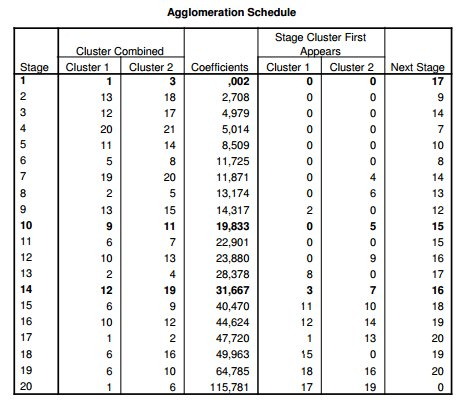
\includegraphics[scale=0.7]{AggloSc}\\
  \caption{SPSS Agglomeration Schedule}
\end{figure}

The procedure followed by cluster analysis at Stage 1 is to cluster the two cases that have the smallest
squared Euclidean distance between them. Then SPSS will recompute the distance measures between all
single cases and clusters (there is only one cluster of two cases after the first step). Next, the 2 cases (or
clusters) with the smallest distance will be combined, yielding either 2 clusters of 2 cases (with 17 cases
unclustered) or one cluster of 3 (with 18 cases unclustered).  This process continues until all cases are clustered into a single group.
For the sake of clarify, we will explain Stages 1, 10, and 14.


\subsubsection{Stage 1}
At Stage 1, Case 1 is clustered with Case 3. The squared Euclidean distance between these two cases is
.002. Neither variable has been previously clustered (the two zeros under Cluster 1 and Cluster 2), and the
next stage (when the cluster containing Case 1 combines with another case) is Stage 17. (Note that at Stage
17, Case 2 joins the Case-1 cluster.)

\subsubsection{Stage 10}
At Stage 10, Case 9 joins the Case-11 cluster (Case 11 was previously clustered with Case 14 back in Stage
5, thus creating a cluster of 3 cases: Cases 9, 11, and 14). The squared Euclidean distance between Case 9
and Case-11 cluster is 19.833. Case 9 has not been previously clustered (the zero under Cluster 1), and
Case 11 was previously clustered at Stage 5. The next stage (when the cluster containing Case 9 clusters) is
Stage 15 (when it combines with the Case-6 cluster).

\subsubsection{Stage 14}
At Stage 14, the clusters containing Cases 12 and 19 are joined, Case 12 has been previously clustered with
Case 17, and Case 19 had been previously clustered with Cases 20 and 21, thus forming a cluster of 5 cases
(Cases 12, 17, 19, 20, 21). The squared Euclidean distance between the two joined clusters is 31.667. Case
12 was previously joined at Stage 3 with Case 17. Case 19 was previously joined at Stage 7 with the Case-
20 cluster. The next stage when the Case-12 cluster will combine with another case/cluster is Stage 16
(when it joins with the Case-10 cluster).

\begin{figure}
  % Requires \usepackage{graphicx}
  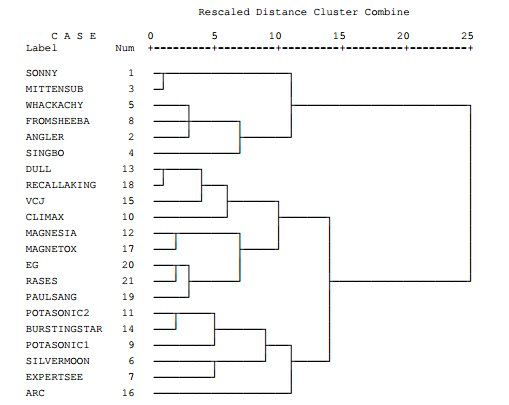
\includegraphics[scale=0.7]{Dendro}\\
  \caption{Corresponding Dendrogram}
\end{figure}

The branching-type nature of the Dendrogram allows you to trace backward or forward to any individual
case or cluster at any level. It, in addition, gives an idea of how great the distance was between cases or
groups that are clustered in a particular step, using a 0 to 25 scale along the top of the chart. While it is
difficult to interpret distance in the early clustering phases (the extreme left of the graph), as you move to
the right relative distance become more apparent. The bigger the distances before two clusters are joined,
the bigger the differences in these clusters. To find a membership of a particular cluster simply trace
backwards down the branches to the name.

\section{Standardizing the Variables}
% % Moved to CA Notes
If variables are measured on different scales, variables with large values contribute
more to the distance measure than variables with small values. In this example, both
variables are measured on the same scale, so that�s not much of a problem, assuming
the judges use the scales similarly. But if you were looking at the distance between two
people based on their IQs and incomes in dollars, you would probably find that the
differences in incomes would dominate any distance measures. (A difference of only
\$100 when squared becomes 10,000, while a difference of 30 IQ points would be only
900. I�d go for the IQ points over the dollars!).

Variables that are measured in large numbers will contribute to the distance more than variables recorded in smaller
numbers.

In the hierarchical clustering procedure in SPSS, you can standardize variables in
different ways. You can compute standardized scores or divide by just the standard
deviation, range, mean, or maximum. This results in all variables contributing more
equally to the distance measurement. That�s not necessarily always the best strategy,
since variability of a measure can provide useful information. 
%----------------------------------------------------- %
\newpage
\section{Non-Hierarchical Clustering}
This method of clustering is very different from the hierarchical clustering and Ward method, which are applied when there is no prior knowledge of how many clusters there may be or what they are characterized by. The k-means clustering approach is used when you already have hypotheses concerning the number of clusters in your cases or variables. For example, you may want to specify exactly three clusters that are to be as distinct as possible.

This is the type of research question that can be addressed by the k-means clustering algorithm. In general, the k-means method will produce the exact k different clusters demanded of greatest possible distinction. Very often, both the hierarchical and the k-means techniques are used successively.
\begin{itemize}
\item Ward's method is used to get some sense of the possible number of clusters and the way they merge as seen from the dendrogram.
\item Then the clustering is rerun with only a chosen optimum number in which to place all
the cases (i.e. k means clustering).
\end{itemize}

In these methods the desired number of clusters is specified in advance and the `best' solution
is chosen. The steps in such a method are as follows:
\begin{itemize}
\item[1] Choose initial cluster centres (essentially this is a set of observations that are far apart
� each subject forms a cluster of one and its centre is the value of the variables for
that subject).
\item[2] Assign each subject to its `nearest' cluster, defined in terms of the distance to the
centroid.
\item[3] Find the centroids of the clusters that have been formed
\item[4] Re-calculate the distance from each subject to each centroid and move observations that
are not in the cluster that they are closest to.
\item[5] Continue until the centroids remain relatively stable.
\end{itemize}

Non-hierarchical cluster analysis tends to be used when large data sets are involved. It is
sometimes preferred because it allows subjects to move from one cluster to another (this is
not possible in hierarchical cluster analysis where a subject, once assigned, cannot move to a
different cluster). Two disadvantages of non-hierarchical cluster analysis are: 
\begin{itemize}
\item[1]it is often
diffcult to know how many clusters you are likely to have and therefore the analysis may have
to be repeated several times 
\item[2] it can be very sensitive to the choice of initial cluster centres. Again, it may be worth trying di?erent ones to see what impact this has.
\end{itemize}

\subsection{Optimal Number of Clusters}
One of the biggest problems with cluster analysis is identifying the optimum number of
clusters. As the joining process continues, increasingly dissimilar clusters must be joined. i.e. the classification becomes increasingly artificial. Deciding upon the optimum number
of clusters is largely subjective, although looking at a dendrogram would help.

% http://www.uk.sagepub.com/burns/data.htm
% Data Set 23 A

% DASL
% http://lib.stat.cmu.edu/cgi-bin/dasl.cgi?query=Cluster+analysis&submit=Search%21&metaname=methods&sort=swishrank



\end{document}

% http://www.uk.sagepub.com/burns/website%20material/Chapter%2023%20-%20Cluster%20Analysis.pdf
% http://www.cs.uu.nl/docs/vakken/arm/additional/additional.html
% Cluster Analysis :  http://www.cs.uu.nl/docs/vakken/arm/SPSS/spss8.pdf
% Discriminant Analaysis : http://www.cs.uu.nl/docs/vakken/arm/SPSS/spss6.pdf
% Factor Analysis : http://www.cs.uu.nl/docs/vakken/arm/SPSS/spss7.pdf




The hierarchical clustering procedure attempts to identify relatively homogeneous groups of cases (or variables) based on selected
characteristics. For example: cluster television shows into homogeneous groups based on viewer
characteristics. In hierarchical clustering, an algorithm is used that starts with each case (or variable) in a
separate cluster and combines clusters until only one is left.



To cluster cases you need to identify variables you wish to be considered in creating clusters for the cases.
The variables to be used for cluster formation are here: picture quality (5 measures), reception quality (3
measures), audio quality (3 measures), ease of programming (1 measure), number of events (1 measure),
number of days for future programming (1 measure), remote control (3 measures), and extras (3 measures).
Pass these in the Variable(s) box.

Cluster Method: Choose the procedure for combining clusters. The default procedure is called the
between-group linkage. SPSS computes the smallest average distance between all group pairs and
combines the two groups that are closest. The procedure begins with as many clusters as there are cases
(here: 21). At step one, the two cases with the smallest distance between them are clustered. Then SPSS
computes distances once more and combines the two that are next closest. After the second step you will
have either 18 individual cases and one cluster of 3 cases, or 17 individual cases and two clusters of two
cases each. The process continues until all cases are grouped into one large cluster.
Measure: Indicate what method is used for distance measuring, the default is Squared Euclidean distance. 

\subsection{Linkage methods}
\begin{itemize}
\item  Single linkage (minimum distance)
\item  Complete linkage (maximum distance)
\item  Average linkage
\end{itemize}

%http://www.rdg.ac.uk/~aes02mm/supermarket.sav

\subsubsection{Ward's method}
\begin{itemize}
\item  Compute sum of squared distances within clusters
\item  Aggregate clusters with the minimum increase in the
 overall sum of squares
\end{itemize}
\subsubsection{Centroid method}
The distance between two clusters is defined as the
 difference between the centroids (cluster averages)